\documentclass{article}

\usepackage{a4wide}
\usepackage{graphicx}
\usepackage{paralist}
\usepackage{hyperref}

\setlength{\parindent}{0em}
\setlength{\parskip}{1em}

\title{Project Information Security: \\ \textbf{Securing an Online Exam}}
\author{Pieter De Baets, Gilles Jacobs, Jasper Van der Jeugt, Toon Willems}

\begin{document}

\makeatletter
\renewcommand\tableofcontents{\@starttoc{toc}}
\makeatother

\maketitle
\tableofcontents

\newpage

\section{Introduction}
\label{sec:introduction}

Asking students to design an exam system is like asking a woodcutter to describe
his perfect axe. Exams are an essential part of our education system and each of
us has pondered the design of an ideal exam system before as it's the target of
our daily activities.

Sadly the contents of exams and interrogation techniques are not part of this
assignment, as we might have some good ideas for that as well. Instead we will
only discuss the technical and practical organisation of exams, and more
specifically exams that are taken over the public internet.

In this report we discuss the challenges and attack vectors that are inherent
with such a setup and provide a practical solution for them.

\section{Requirements and Architecture}
\label{sec:requirements}

We chose to design a system with a central component, i.e. a server, to which
the different clients can connect. For users, it would appear that this central
server is their exam platform. This is not true however, as responsibilities and
software is distributed over all platform participants.

One disadvantage of this approach is that this server needs to be trusted to
some extent by the users, which we tried to limit as much as possible.

\subsection{Assumptions}
\label{subsec:req-assumptions}

We need to assume that every user (students as well as professors) are
registered on this platform. These accounts can be created when a student
enrolls in the institute, or when a professor is employed.

The users of the platform should be able to verify that they are indeed talking
to the official platform instance, and not to some attacker posing as the
platform. This problem is mostly alleviated by using HTTPS with a trusted
cerficate for all communication.

We use asymmetric encryption mechanisms for many features, so we also need to
assume that each user has a keypair assigned. These keypairs can be created at
the same time as the accounts, with some option to reset a keypair when it has
been compromised. The platform only requires a user's public key, the private
key is to be kept secret by the user.

Ideally these keys are also signed by an official entitity so that users can
lookup and trust public keys found through a public key exchanges.

\subsection{Functionality}
\label{subsec:req-functionality}

\subsubsection{Logging in}

Users (students and professors) should be able to log in to the application,
prove their identity and receive the correct permissions. This means we need
some kind of authentication: it is obvious that a student should not be able to
pose as a professor and modify an exam, or submit answers as another student.

\subsubsection{Setup and distribution of exams}

The professor needs to be able to distribute an exam to the students. He first
uploads it to the central server, and selects a number of students. These
students can download it from there, at some point in time, also specified by
the professor.

Integrity is important here: we must ensure the students see the same exam that
the professor posted without any alterations. Furthermore, only the selected
students should be able to see the exam, and we have to make sure they cannot
view the exam before they are allowed to.

Another goal of the exam platform is to simplify the disclosure of the exam
questions for the professor. We provide 2 solutions for this:

\begin{enumerate}

\item \textbf{Timed exam release}: when setting up the exam, the professor can
choose the period of time during which the exam should be available to selected
students. Outside this time period the system will not allow any access to the
data.

\item \textbf{Locked exams}: as storing the exam unencrypted on the server is a
potential, albeit small, risk (see \autoref{subsec:req-attacks}), we provide the
professor with the additional option of uploading an encrypted version of the
exam, which the system can unlock later when a passphrase is given.

This is a minor action that can be done a couple of hours in advance of the
exam, and which provides an extra layer of security around the exam data.

\end{enumerate}

Finally, when students download the exam, they need to receive some form of
proof of their interaction with the server as part of the audit trail. This
might not be very important in this phase of the exam procedure but it will be
in the next section.

\subsubsection{Receving answers from students}

% To discuss:
% * should be impossible to alter answers
% * only professor can read them
% * student needs proof of submission by server
After completion of an exam, the student can upload his answers to the server
by viewing an exam on the platform, and choosing the upload answers option.
After uploading his answers, the student receives a proof of submission from
the server.

When a student uploads his answers, we have to ensure these answers are not
altered and that only the professor can read these answers.

Later, the professor can download the answers of his students and revise the
answers to calculate the results.

\subsubsection{Distributing exam results}

% To discuss:
% * only student can see his result
% * student should be able to verify that professor authored resuls
Finally, when the professor has the results of a student's exam answers, he
can upload them to the server.

It is important that these results can only be viewed by the student 
they are intended for, and that they are authored by the professor.

\subsection{Expected attacks}
\label{subsec:req-attacks}

How will attackers try to compromise our system? Why will they fail?

Passive attacks, active attacks, passive-aggressive attacks, you name 'em, we
got 'em.

\begin{itemize}
\item Impersonating the exam-server
\item Man in the middle
\item Sniffing traffic
\item Attacks on the platform: SQL injection, CSRF, XSS
\item ...
\item Time attack: early exam release due to NTP attacks
\item Malicious system administrator: can access server fs, remo
\end{itemize}

\subsection{Limitations}
\label{subsec:req-limitations}

In what ways is our system not protected? What do we need to trust for the
system to work?

\section{Practical considerations}
\label{sec:practical}

Is it practically feasible to lock up a few dozen students in a small room for a
few days, without food or water?

\section{Concrete implementation}
\label{sec:implementation}

Some implementation details, we should mention the actually used algorithms
here.

\subsection{Authentication}
\label{subsec:impl-authentication}

It is definitely possible to design a custom secure authentication solution.
However, given the setting, we chose for a more realistic option. Most large
organisations have an in-house authentication gateway which applications can
use. This way authentication can be organised securely across the whole
organisation without much effort to application developers.

For our proof-of-concept we integrated with Ghent University's Central
Authentication Server\footnote{\url{http://helpdesk.ugent.be/webhosting/en/cas.php}}
(CAS) which is an implementation of the publicly available CAS
protocol\footnote{\url{http://www.jasig.org/cas/protocol/}}. The basic
exchange of messages between user, CAS server and application server can be seen
in figure \ref{fig:login} and is detailed below.

\begin{figure}[ht]
  \begin{center}
  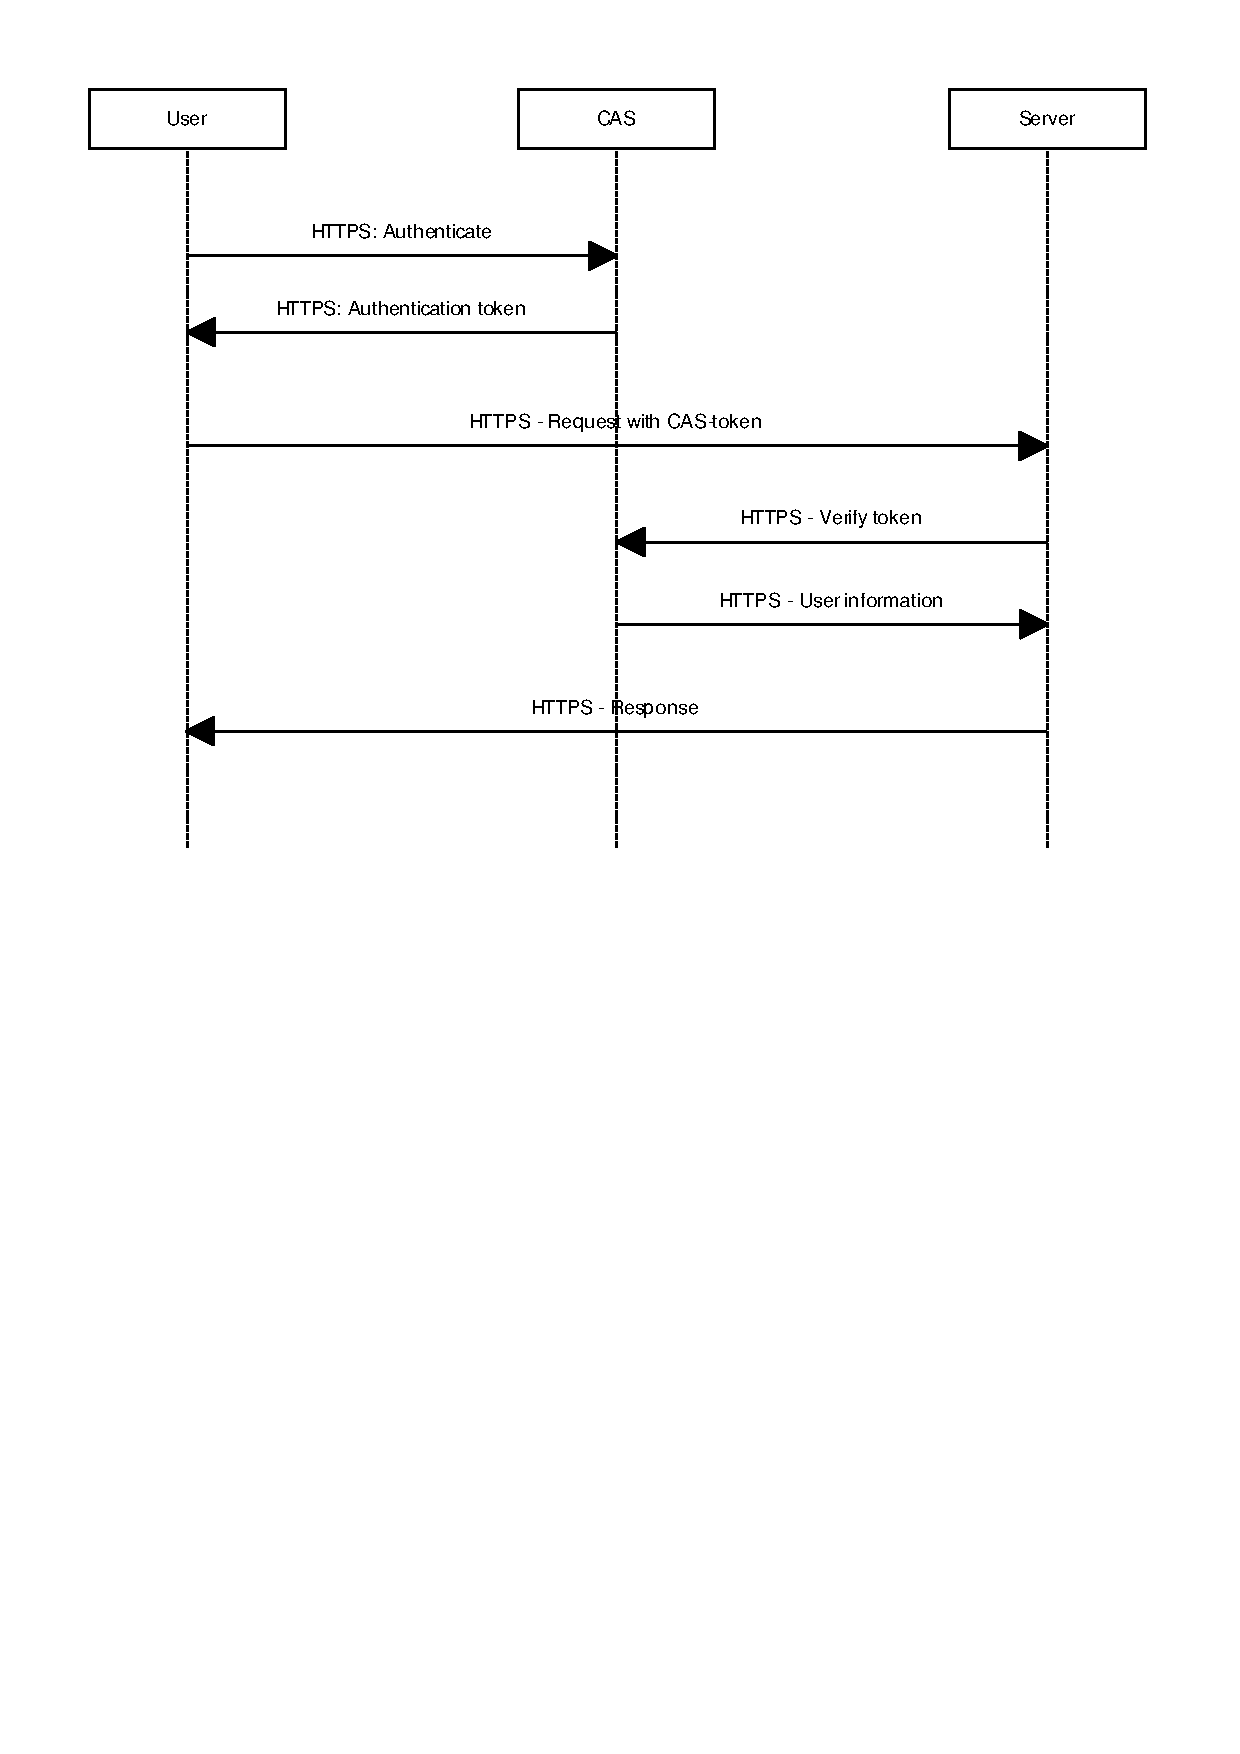
\includegraphics[width=0.9\textwidth]{images/login.pdf}
  \caption{Messages exchanged when logging in}
  \label{fig:login}
  \end{center}
\end{figure}

\begin{enumerate}
\item The user has no active session on the exam server and is redirected
  to the authentication server (referencing the exam server as source of the
  authentication request).
\item The authentication server verifies the identify of the user. In Ghent
  University's case, this is a basic password authentication scheme (in which
  hopefully a secure hash of the password is used instead of a plaintext
  version), but more advanced options (e.g. smart cards, biometrics, ...) are
  possible as well.
\item When authentication has succeeded the authentication server generates
  a security token and returns the user to the exam server, carrying this token.
\item The exam server will then contact the authentication server and confirm
  the user's identity by using this token. The use of the token is strictly
  regulated to prevent abuse: only the requesting service can use it, it is only
  valid during a small timeframe and can only be used once.
\item Having received this information, the exam server can now start a local
  application session for the authenticated user.
\end{enumerate}

\subsection{Exam distribution}
\label{subsec:impl-exams}

When a user wants to upload, unlock or download an exam we assume that he is
already autenticated with the platform, as explained in
\autoref{subsec:impl-authentication}.

\begin{enumerate}
\item Upload: when uploading an exam the professor sends a file, containing
  the examination and a signature, and encrypted with the private key of the
  professor (\autoref{fig:upload-exam}).
\item Unlock: the professor can unlock a locked exam by sending a symmetric key
  (\autoref{fig:unlock-exam}).
\item Download: when a student downloads an exam, the server sends the
  exam and its signature, as well as a proof of interaction with the server
  and its signature (\autoref{fig:download-exam}).
\end{enumerate}

\begin{figure}
  \begin{center}
  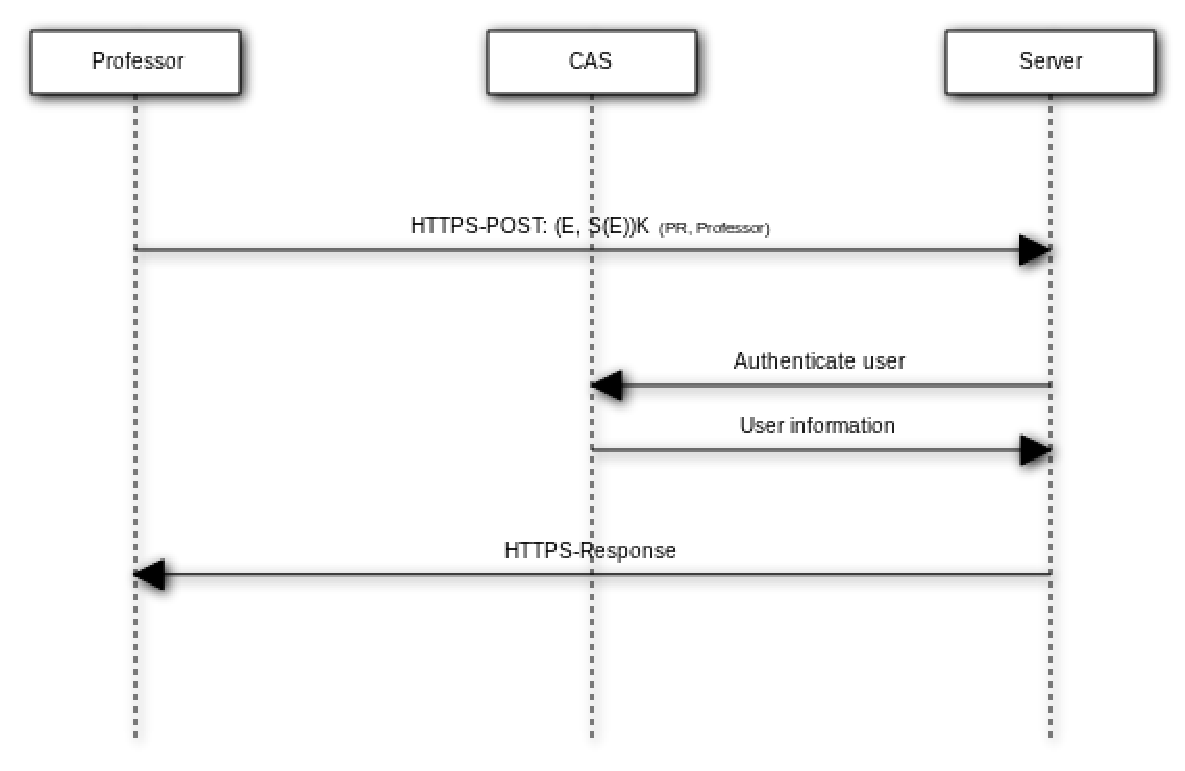
\includegraphics[width=0.75\textwidth]{images/upload_exam.pdf}
  \caption{Messages exchanged when uploading an exam}
  \label{fig:upload-exam}
  \end{center}
\end{figure}

\begin{figure}
  \begin{center}
  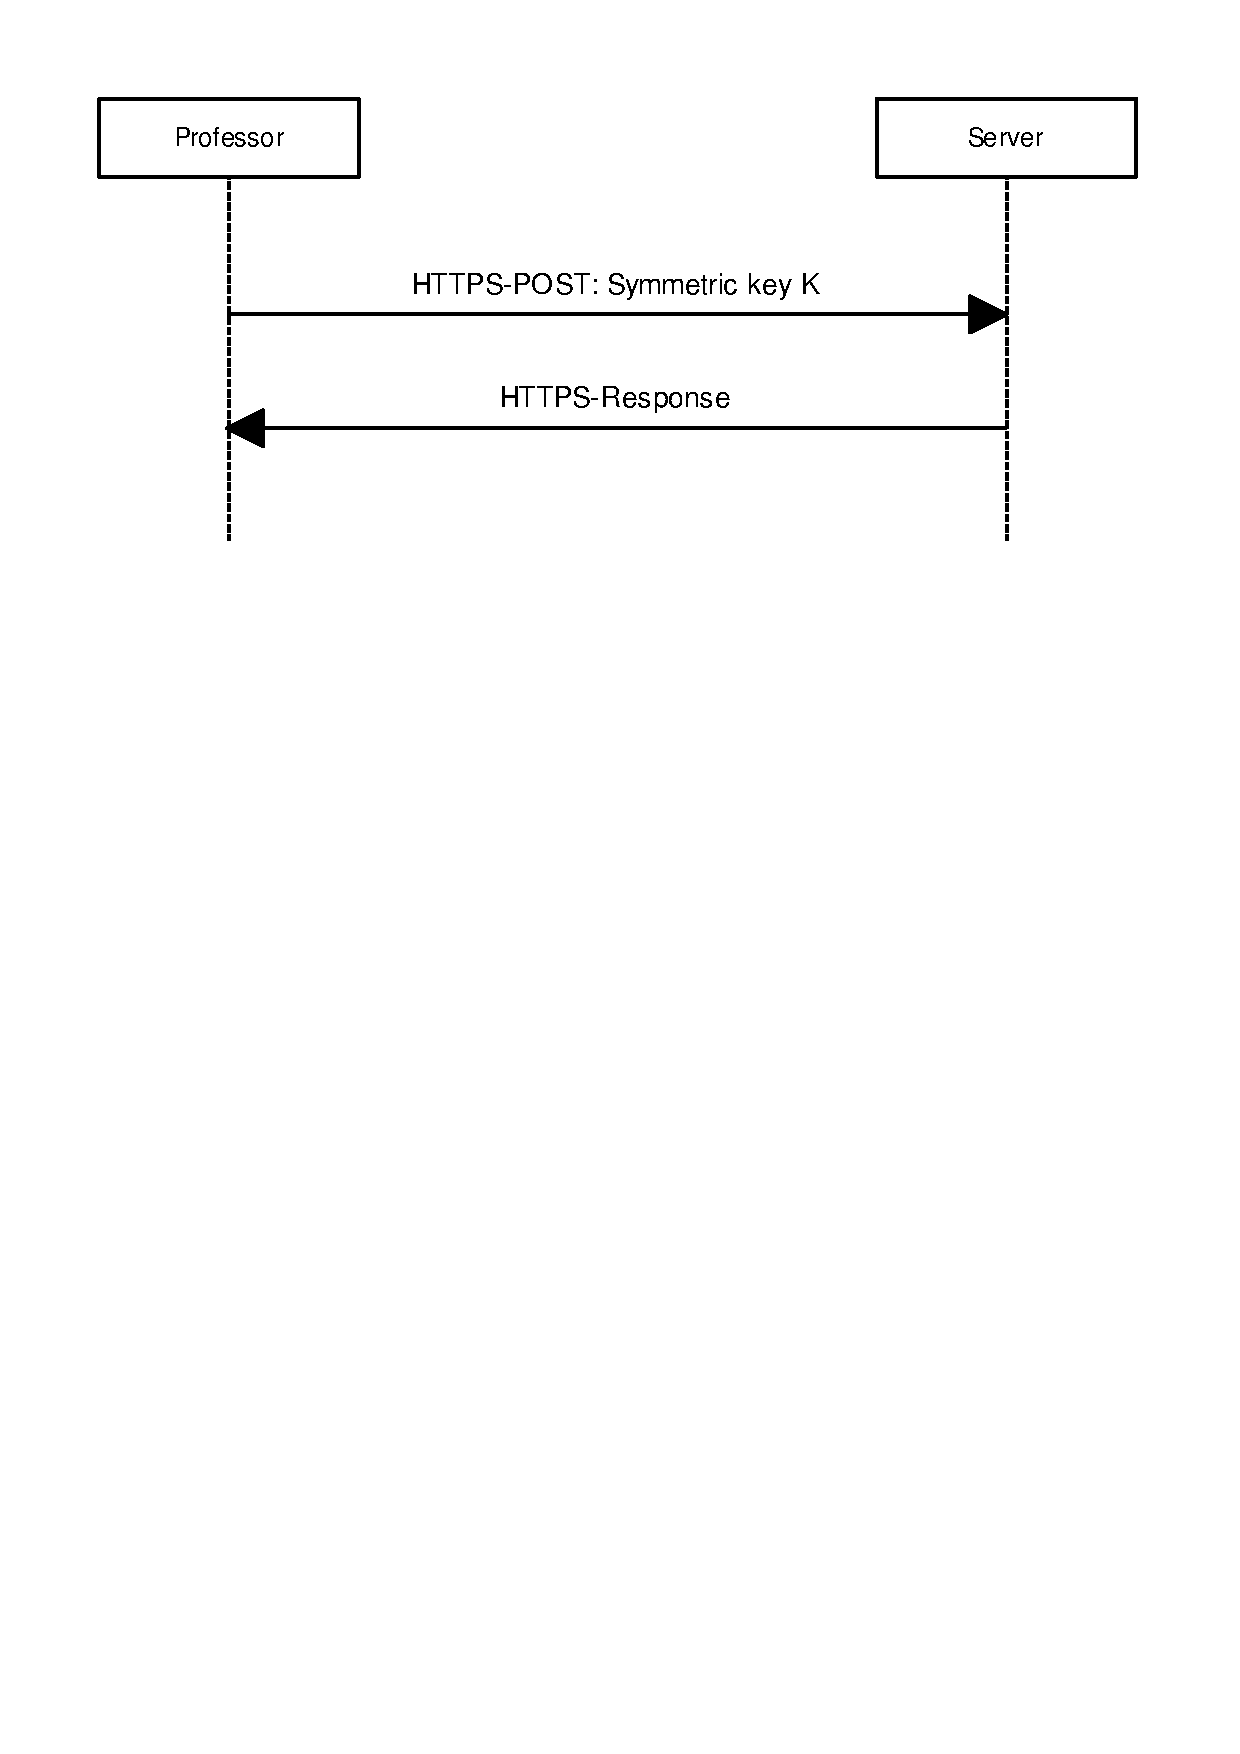
\includegraphics[width=0.75\textwidth]{images/unlock_exam.pdf}
  \caption{Messages exchanged when unlocking an exam}
  \label{fig:unlock-exam}
  \end{center}
\end{figure}

\begin{figure}
  \begin{center}
  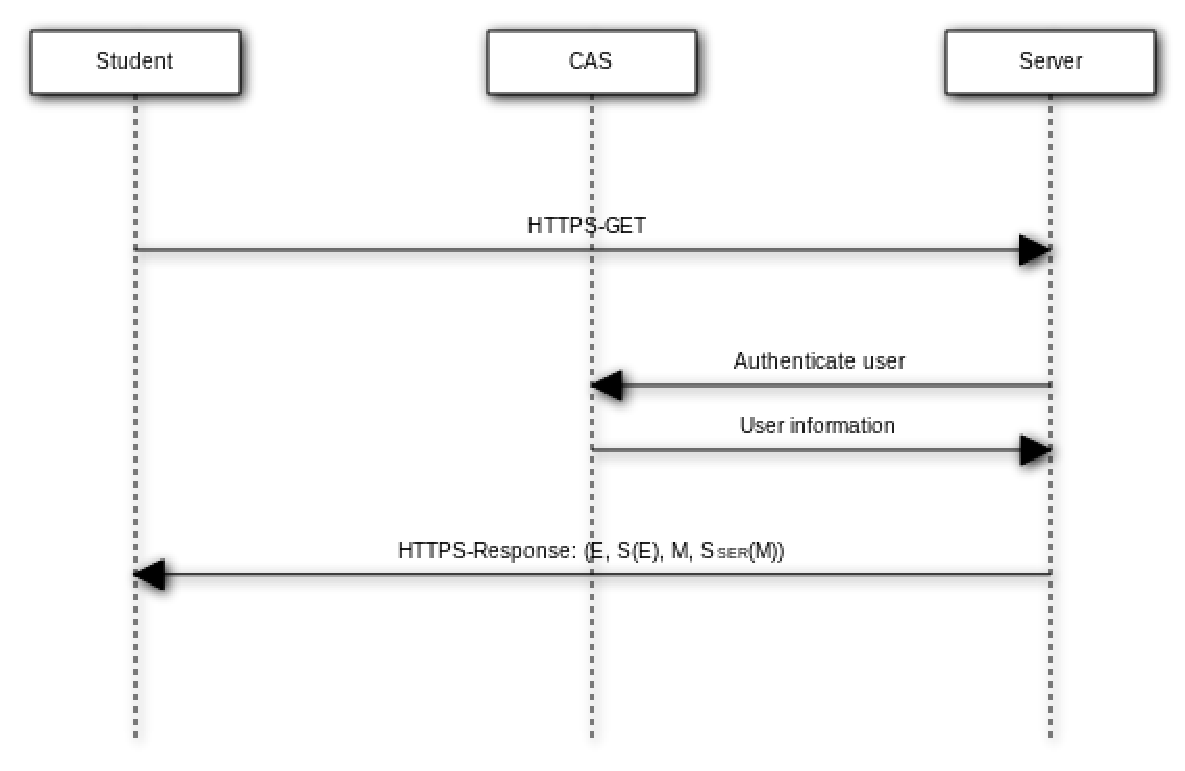
\includegraphics[width=0.75\textwidth]{images/download_exam.pdf}
  \caption{Messages exchanged when downloading an exam}
  \label{fig:download-exam}
  \end{center}
\end{figure}

\subsection{Receving answers from students}
\label{subsec:impl-answers}

When a user wants to upload or download an exam answers we assume that he is
already autenticated with the platform, as explained in
\autoref{subsec:impl-authentication}.

\begin{enumerate}
\item Upload: (\autoref{fig:upload-answers}).
\item Download: (\autoref{fig:download-answers}).
\end{enumerate}

\begin{figure}
  \begin{center}
  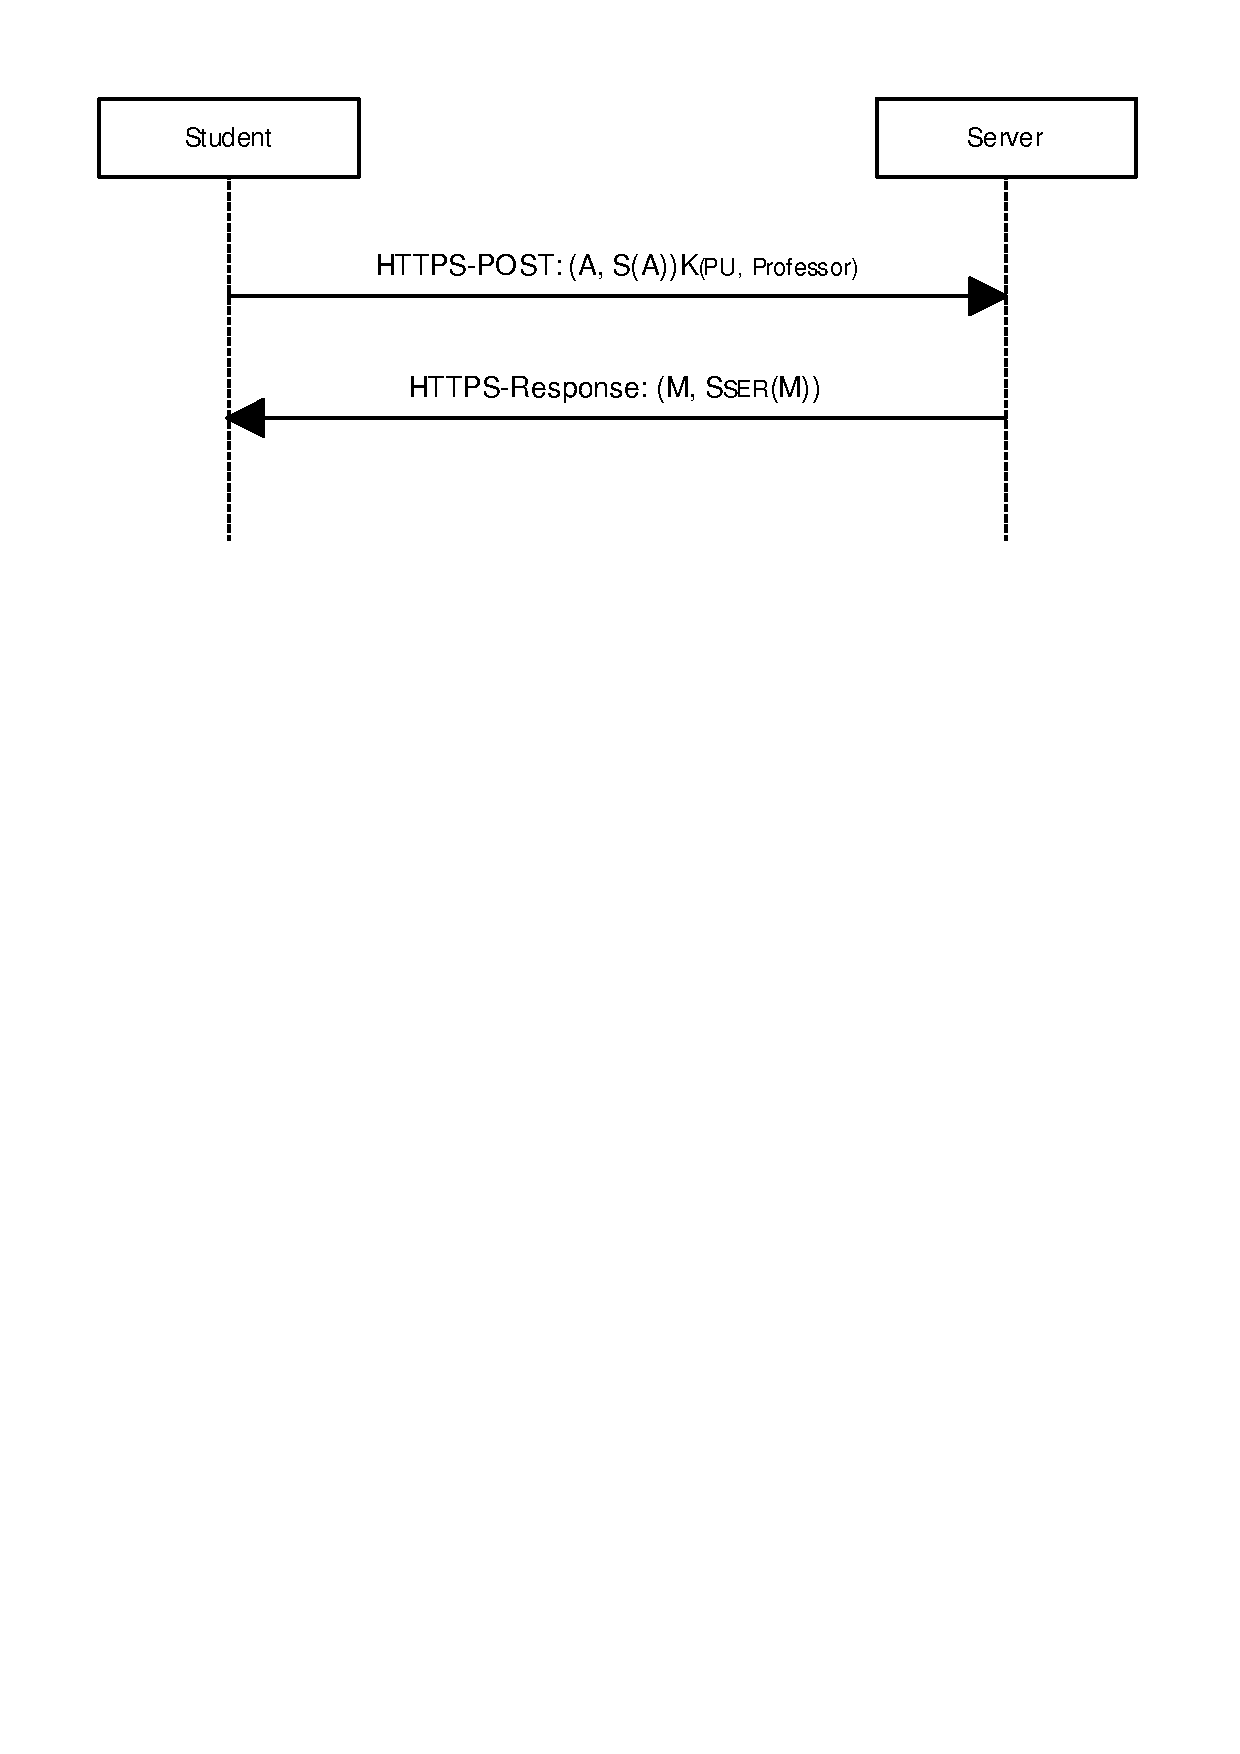
\includegraphics[width=0.75\textwidth]{images/upload_answers.pdf}
  \caption{Messages exchanged when uploading answers}
  \label{fig:upload-answers}
  \end{center}
\end{figure}

\begin{figure}
  \begin{center}
  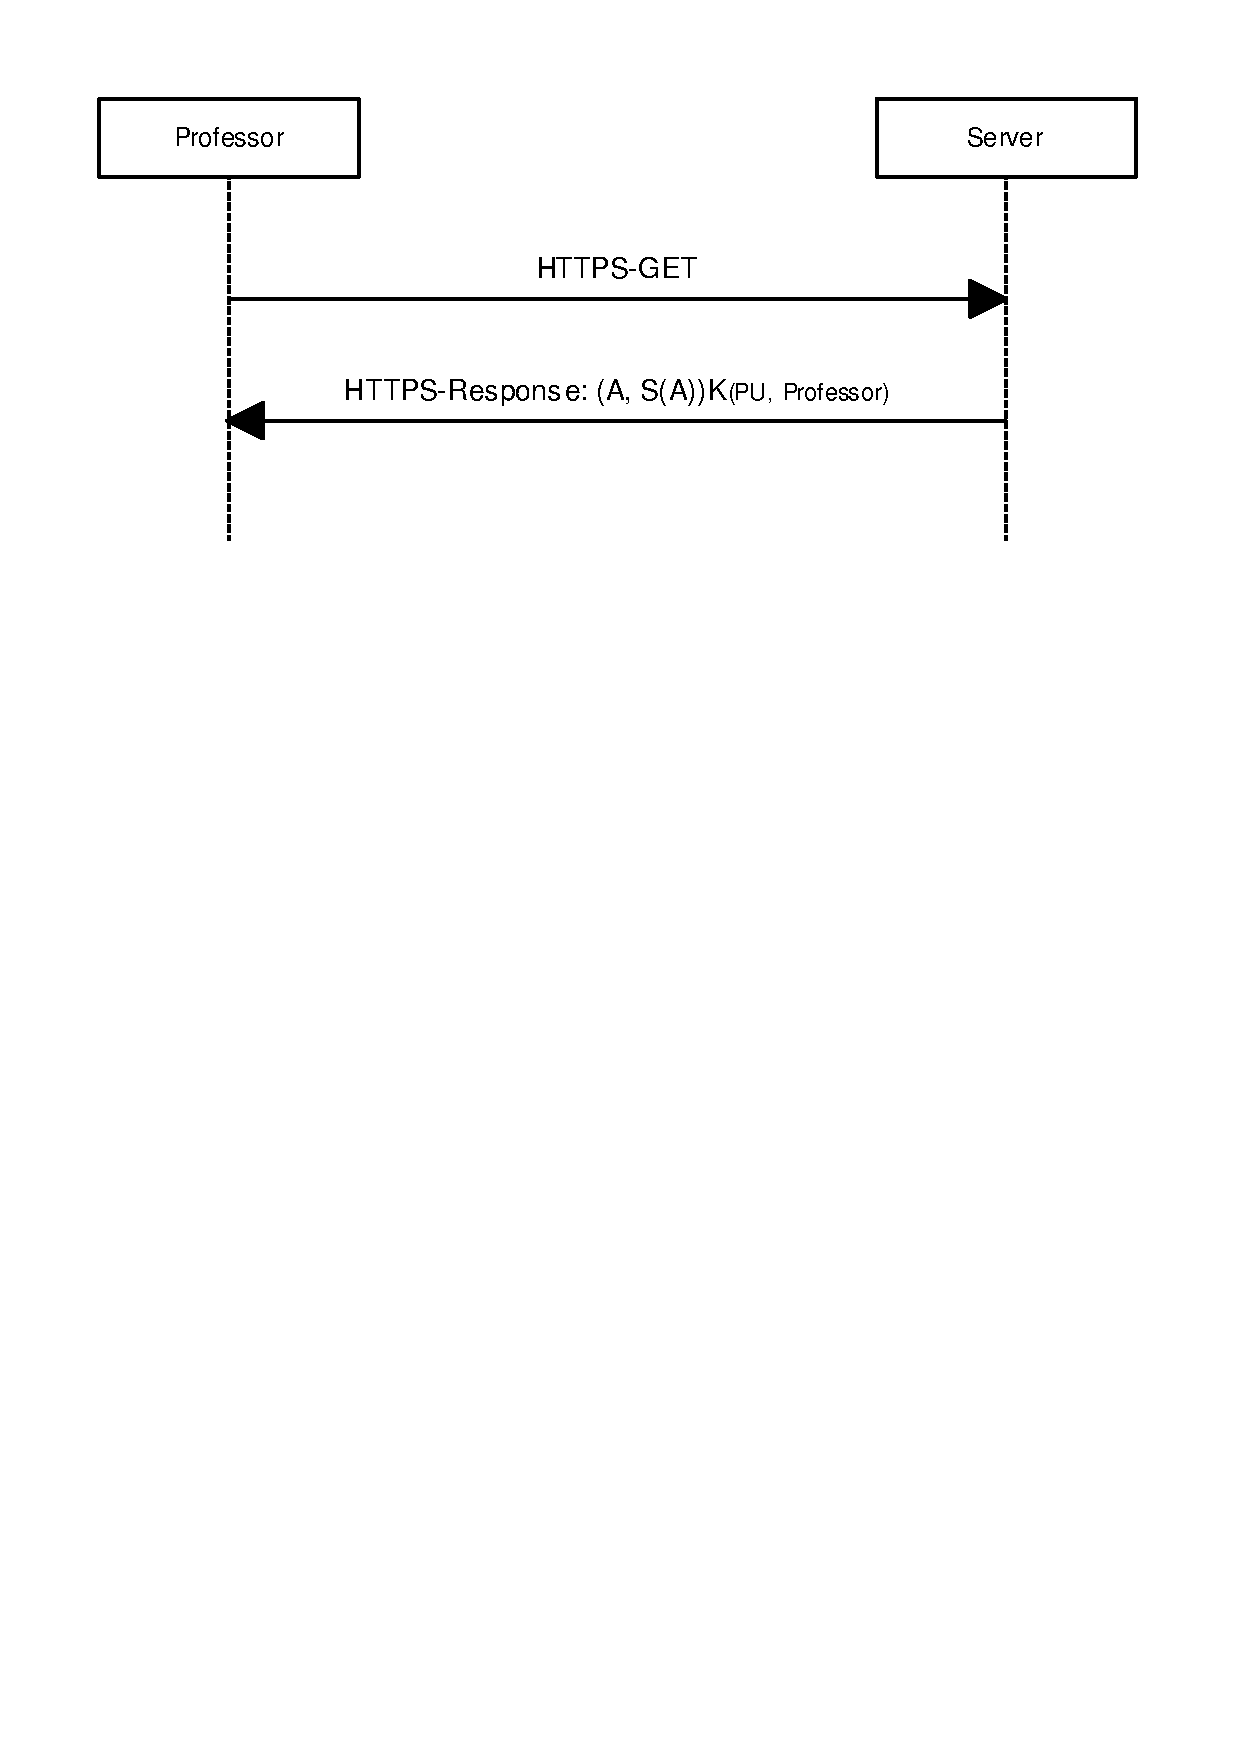
\includegraphics[width=0.75\textwidth]{images/download_answers.pdf}
  \caption{Messages exchanged when downloading answers}
  \label{fig:download-answers}
  \end{center}
\end{figure}

\subsection{Distributing exam results}
\label{subsec:impl-results}

\begin{figure}
\begin{center}
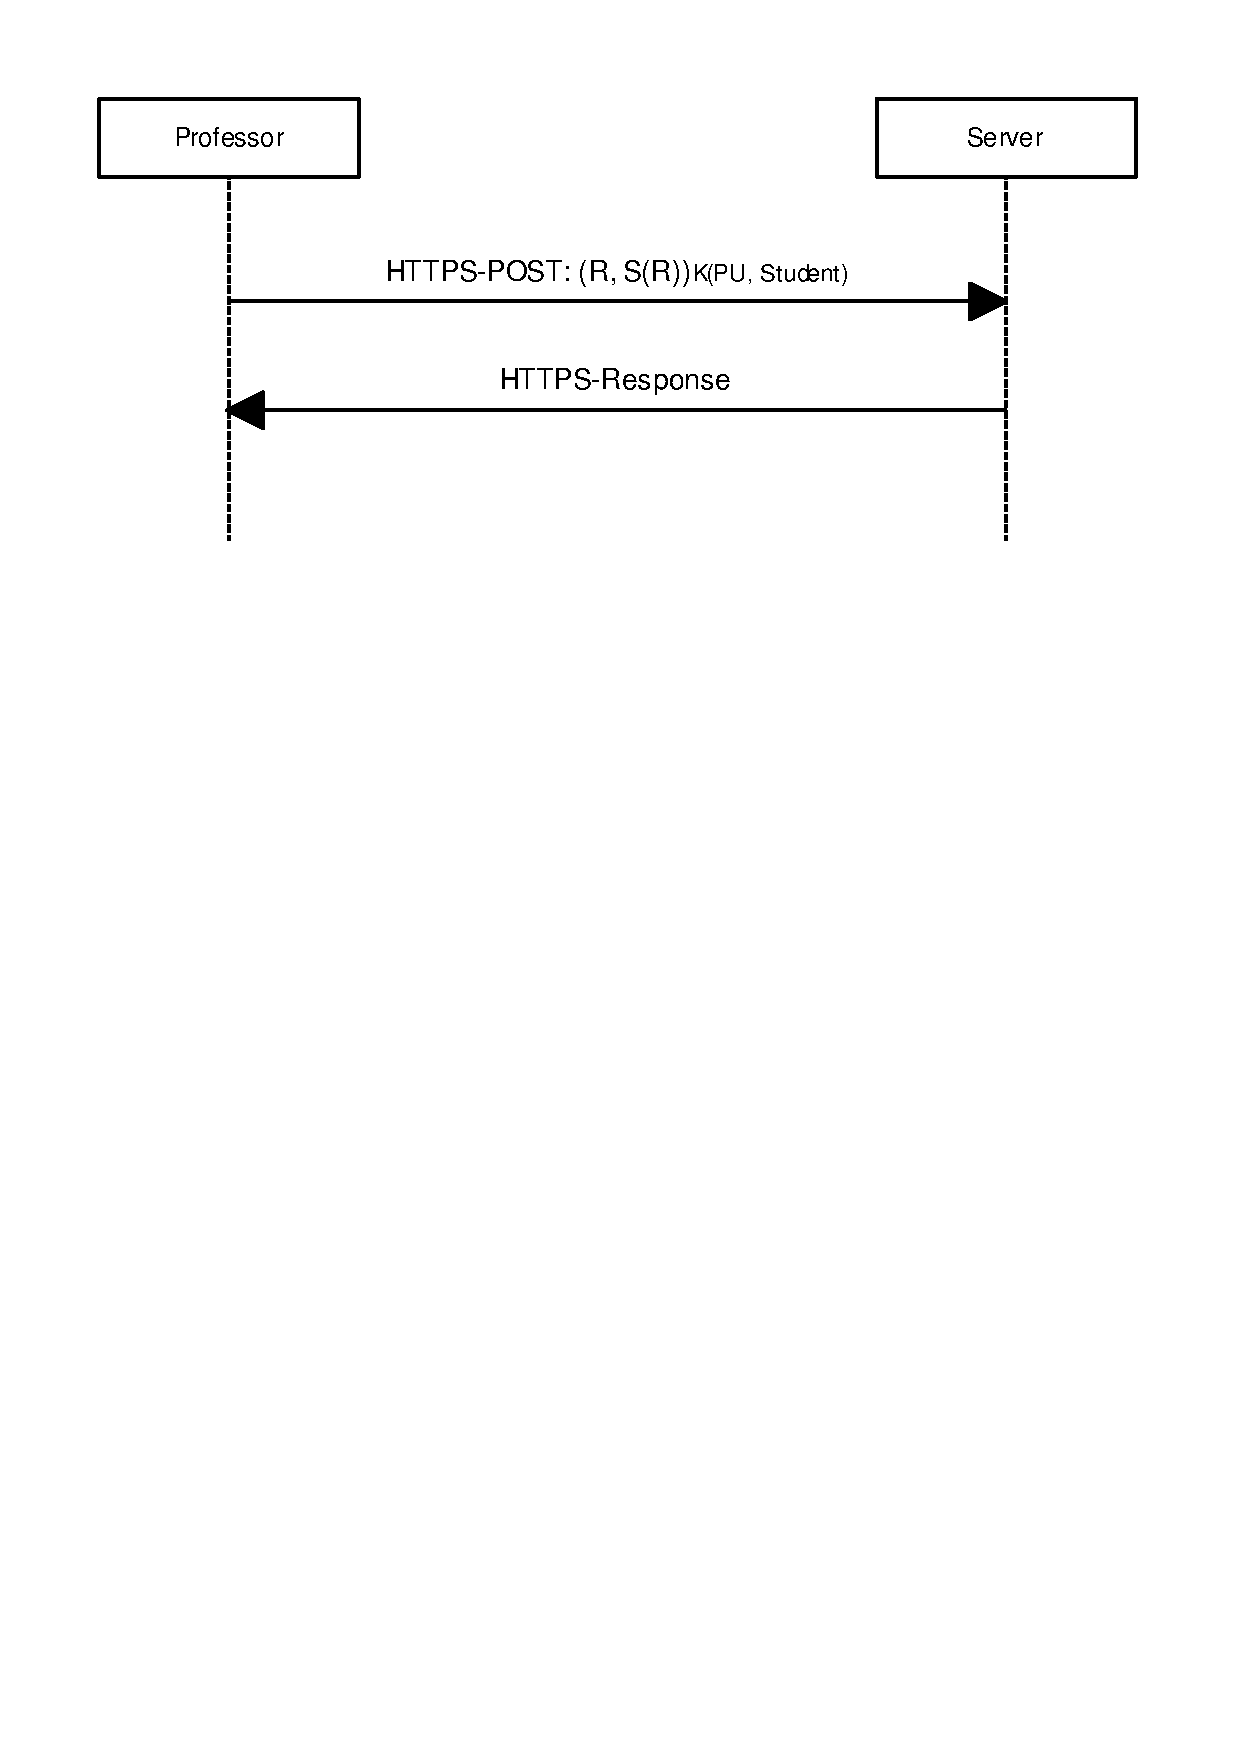
\includegraphics[width=0.75\textwidth]{images/upload_scores.pdf}
\caption{Messages exchanged when uploading scores}
\label{fig:upload-scores}
\end{center}
\end{figure}

\begin{figure}
\begin{center}
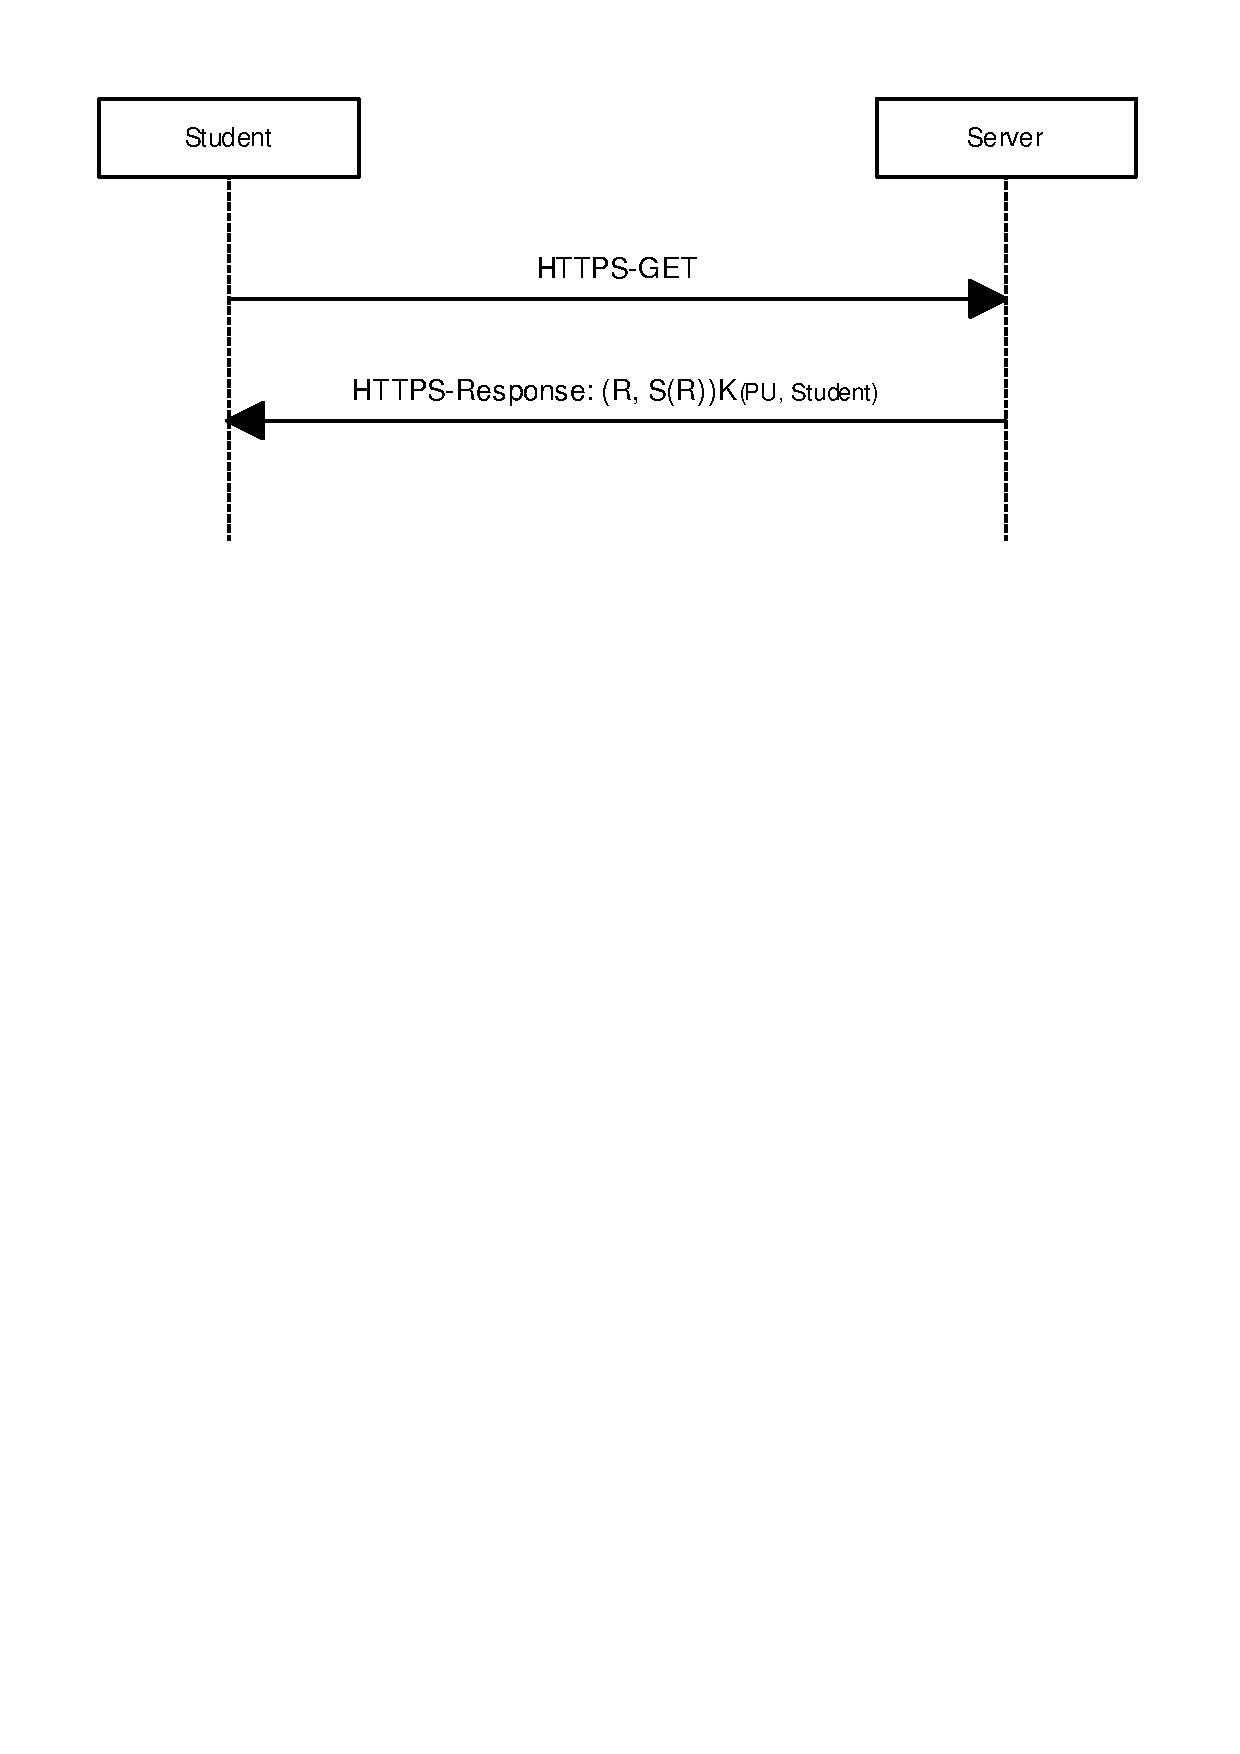
\includegraphics[width=0.75\textwidth]{images/download_scores.pdf}
\caption{Messages exchanged when downloading scores}
\label{fig:download-scores}
\end{center}
\end{figure}


\section{Conclusion}
\label{sec:conclusion}

INSERT +8000 WORDS HERE.

\end{document}
